\chapter{DC Circuits}

\section{Introduction}

In this lab, you will learn how to use your digital multimeter (DMM) and bench-top DC power supply to explore DC circuits involving resistors.  You will experimentally verify Ohm's law and the equivalent resistance for resistors in series and parallel.  You will solder two resistor circuits to explore the $\Delta$-$Y$ transformation for three terminal networks.

\section{Benchtop Power Supply}
% MASTECH HY3005F-3

\section{Digital Multimeter}
% Triplett 9007 (often blown fuse)
% Mastech MS8264 (resettable fuse)

\begin{figure}[htbp]
\begin{center}
\begin{tabular}{c@{\hskip 2cm}c}

\begin{circuitikz}[line width=1pt]
\draw (0,0) to[battery1,bipoles/length=1.5cm] ++(0,+4.0) to[short] ++(2.0,0) coordinate(A);
\draw (A) to[resistor,l_=$R_1$] ++(0,-2.0) to[short] ++(0,-2.0) to[short] ++(-2,0);
%node[ground,yscale=2.0]{};
\draw (0,1.7) node[left]{$-$};
\draw (0,2.4) node[left]{$+$};
\draw (A) to[short,*-] ++(2.0,0.0) to[short] ++(0.0,-1.0) node[component]{V} to[short] ++(0.0,-1.0) to[short,-*] ++(-2.0,0);
\end{circuitikz} &

\begin{circuitikz}[line width=1pt]
\draw (0,0) to[battery1,bipoles/length=1.5cm] ++(0,+4.0) to[short] ++(2.0,0);
\draw (A) to[resistor,l_=$R_1$] ++(0,-2.0) to[short] ++(0,-1.0) 
node[component]{A} to[short] ++(0,-1.0) to[short] ++(-2.0,0);
%node[ground,yscale=2.0]{};
\draw (0,1.7) node[left]{$-$};
\draw (0,2.4) node[left]{$+$};
\end{circuitikz} \\

(a) & (b) \\
\end{tabular}
\caption{Circuits for verifying Ohm's law.}
\label{fig:dmmscematic}
\end{center}
\end{figure}




% Triplett 9007 (often blown fuse)
% Mastech MS8264 (resettable fuse)
% Wish Board No.  206
% MASTECH HY3005F-3

In this lab, you will use two new pieces of lab equipment:  your bench-top power supply and your digital multimeter (DMM).

Your bench-top supply provides up to XX volts of DC power on two independent channels.  For this lab, we'll only be using a single channel.  Each supply has two associated knobs, one controlling the maximum allowed current, and one controlling the maximum voltage.  The supply will provide the maximum voltage subject to those constraints.  Usually your are primarily concerned with setting the voltage by the voltage knob, but it is a good habit, which will save you from losing components, to set the current as low as possible.  An LED indicates if your circuit is current limited or voltage limited.  You can adjust the current limit until just beyond the point where your circuit become voltage limited.

The supply is floating, it provides the specified voltage between the black and red outputs without referencing either to ground.  If you want to provide a ground referenced voltage you explicitly connect the green output to the red (positive) terminal or the black (negative) terminal.

(Discuss limits)

Your DMM can measure voltage, resistance, and current.






\section{Verification of Ohm's Law}

\begin{figure}[htbp]
\begin{center}
\begin{tabular}{c@{\hskip 2cm}c}

\begin{circuitikz}[line width=1pt]
\draw (0,0) to[battery1,bipoles/length=1.5cm] ++(0,+4.0) to[short] ++(2.0,0) coordinate(A);

\draw (A) to[resistor,l_=$R_1$] ++(0,-2.0) to[short] ++(0,-1.0) 
node[component]{A} to[short] ++(0,-1.0) to[short] ++(-2.0,0);
%node[ground,yscale=2.0]{};
\draw (0,1.7) node[left]{$-$};
\draw (0,2.4) node[left]{$+$};
\draw (A) to[short,*-] ++(2.0,0.0) to[short] ++(0.0,-1.0) node[component]{V} to[short] ++(0.0,-1.0) to[short,-*] ++(-2.0,0);
\end{circuitikz} &
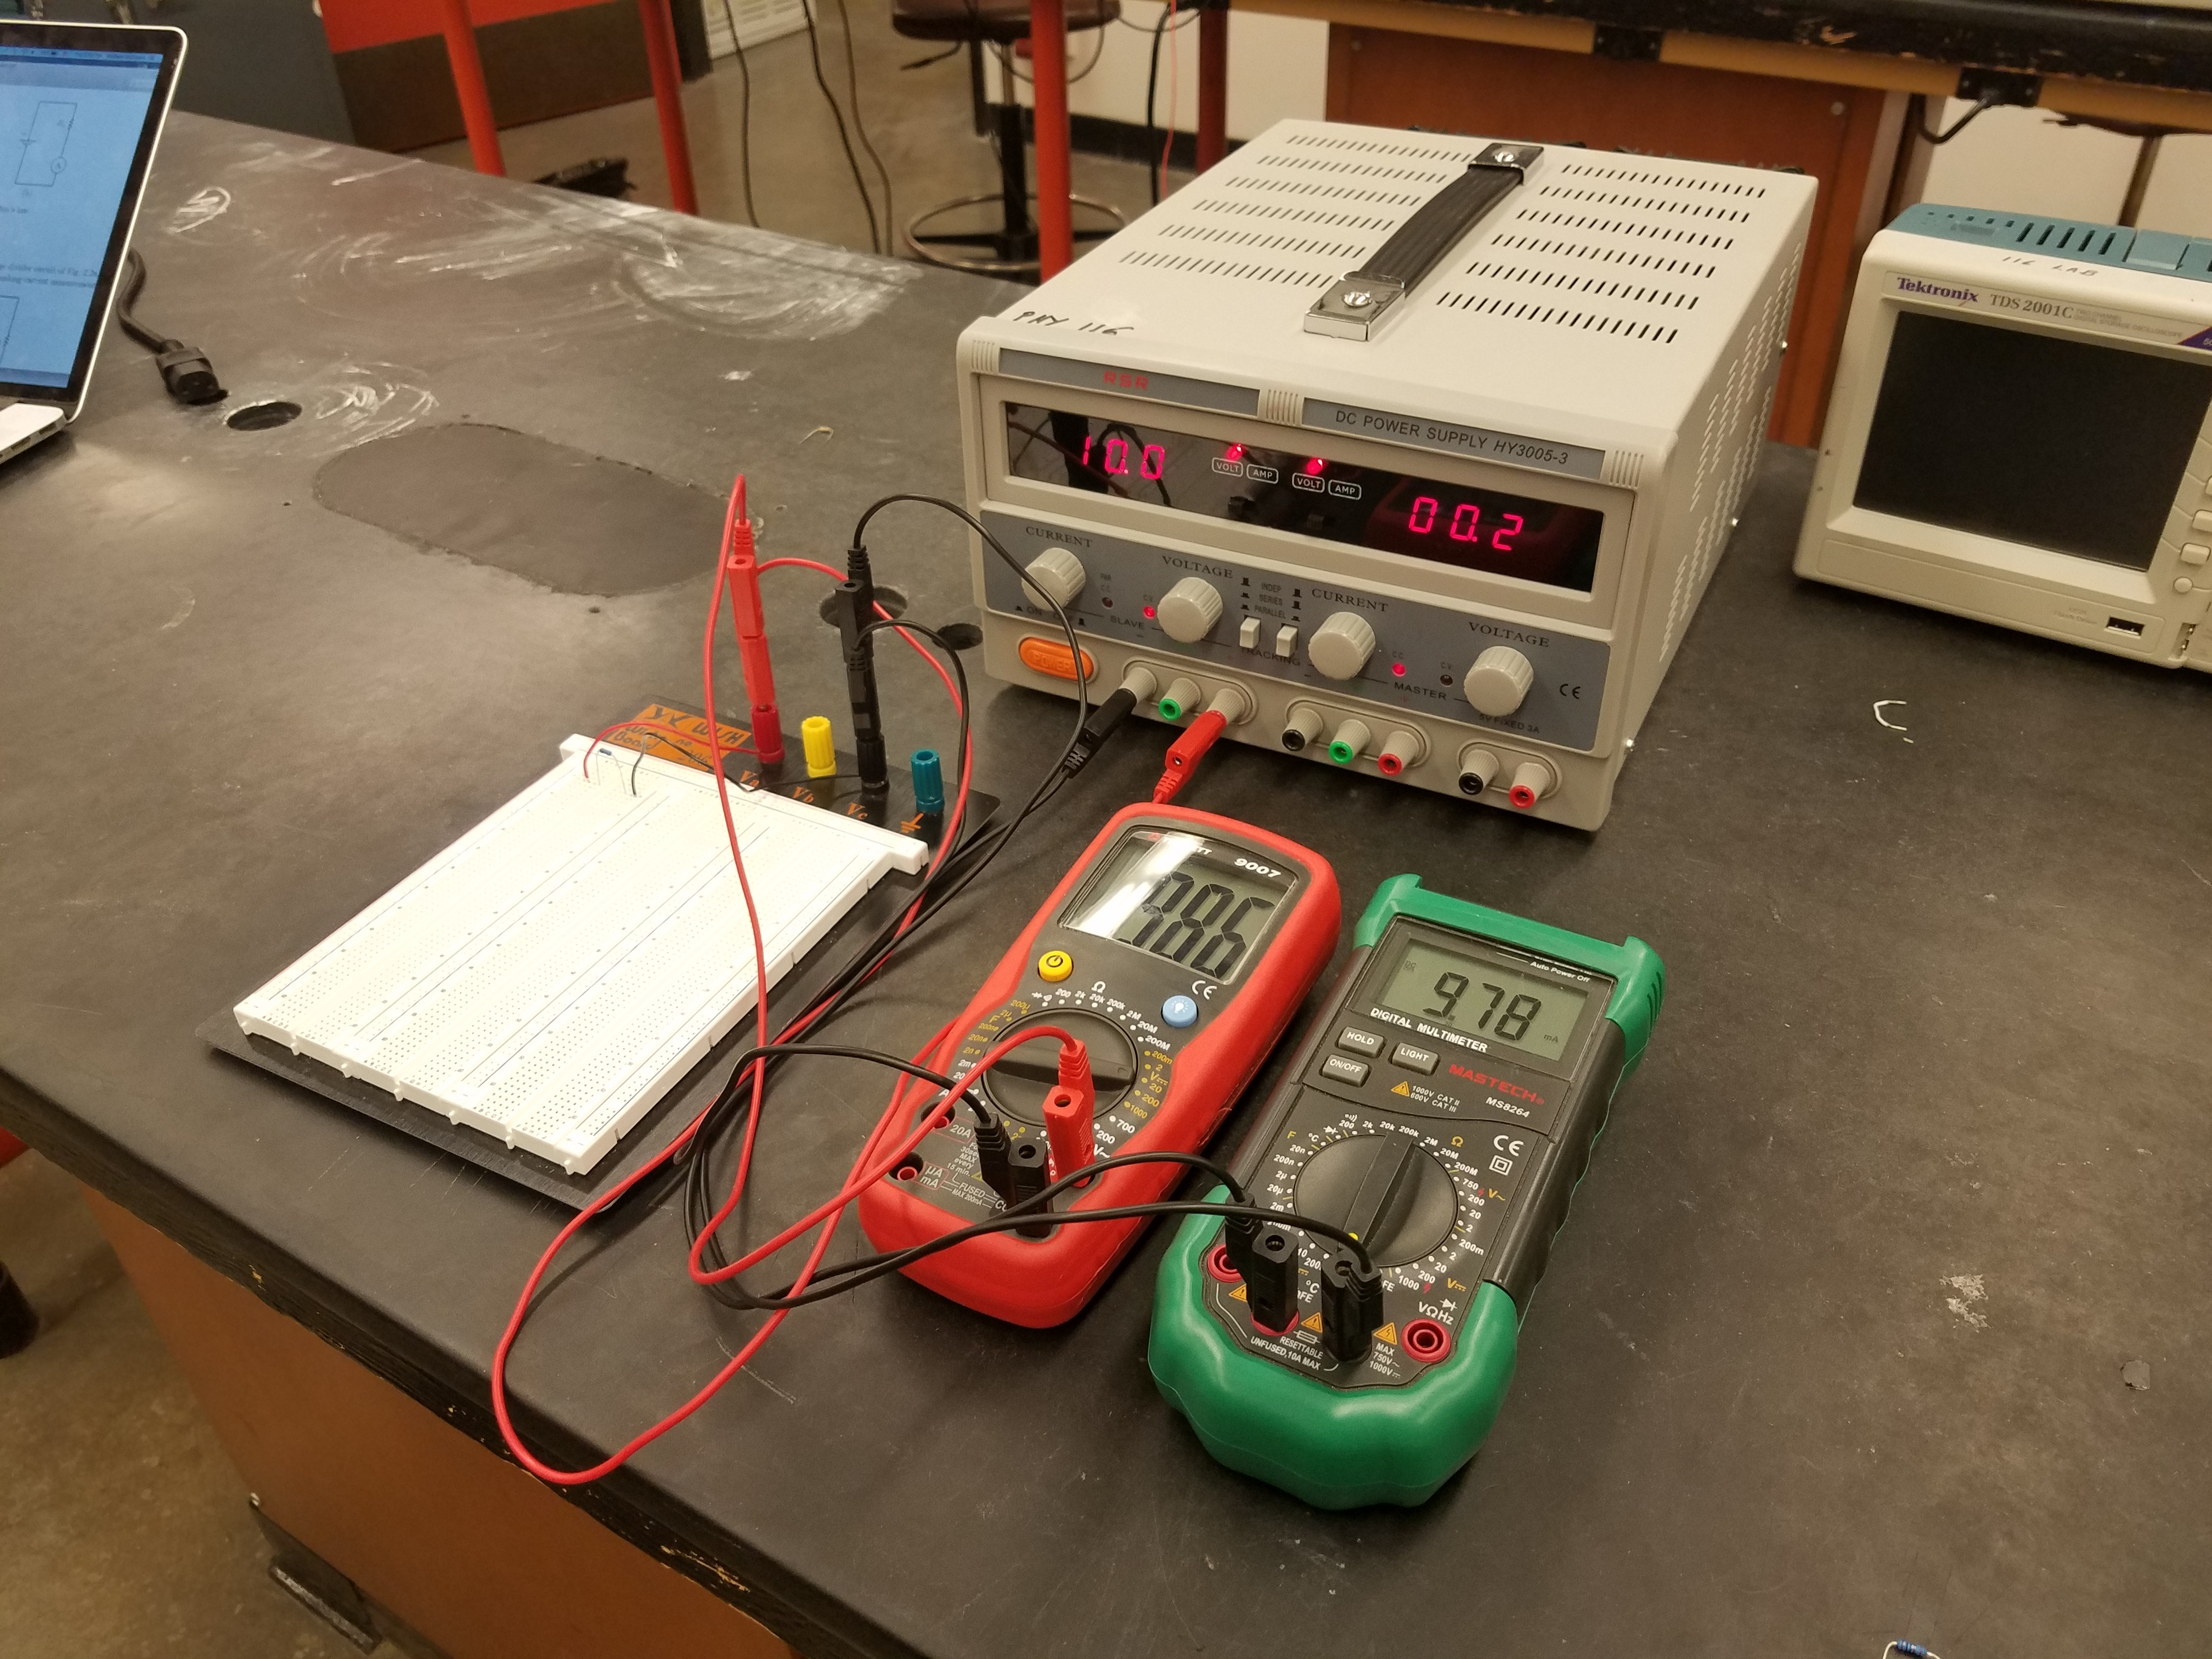
\includegraphics[height=0.25\textheight]{figs/labs/dc_circuits/setup.jpg} \\
(a) & (b) \\
\end{tabular}
\caption{Circuit for verifying Ohm's law as a (a) circuit diagram, and (b) implemented using your lab equipment.}
\label{fig:ohmslaw}
\end{center}
\end{figure}


Build the circuit in Fig.~\ref{fig:ohmslaw}.  Use a resistor $R_1 = 1.0~{\rm k\Omega}$ with a $1\%$ tolerance.  Use your Triplett 9007 as the voltmeter and the Mastech MS8624 as the current meter.  Use your benchtop power supply to provide the voltage.  

By adjusting the voltage setting of the power supply, take a series of voltage and current measurements with voltage across the resistor at target voltages from $1$ to $10~\rm V$ in steps of $1~\rm V$.   Generally, you can measure more precisely than you can control, so never fuss about trying to measure the voltage at exactly the target value, instead, simply record e.g. $V=1.04~\rm V$ along with your current measurement and move on to the next target value.

While recording data, check that the current values you measure are consistent with what you expect given the voltage across the resistor and resistance.  You should {\em always} make quick sanity calculations when collecting data, otherwise you risk wasting time collecting useless data!

{\bf Plot 1:}  Plot the current versus voltage of your ten data points (using option {\tt "o"}).  Draw a line (using option {\tt "-"}) for the current versus voltage curve of a $1.0~\rm k\Omega$ resistor.  Make certain your plot has appropriate axis labels, including appropriate units in parenthesis, and a legend distinguishing data from your expectation (``expected").  {\bf Measurement 1:}  After taking your last measurement, leave all the connections in place and the power-supply at $10~\rm V$.  Record in your log book the resistance of the resistor $R_1$ reported by your DMM.  Is this a reasonable measurement?  {\bf Measurement 2:}  Turn off the DC supply and record the resistance reported by the DMM.  Is this accurate?  {\bf Measurement 3:}  Remove the resistor from your circuit and measure the resistance with your DMM.  Is this accurate?

\begin{figure}[htbp]
\begin{center}
\begin{tabular}{c@{\hskip 2cm}c}

\begin{circuitikz}[line width=1pt]
\draw (0,0) to[battery1,bipoles/length=1.5cm] ++(0,+4.0) to[short] ++(2.0,0) coordinate(A);
\draw (A) to[resistor,l_=$R_1$] ++(0,-2.0) to[short] ++(0,-2.0) to[short] ++(-2,0);
%node[ground,yscale=2.0]{};
\draw (0,1.7) node[left]{$-$};
\draw (0,2.4) node[left]{$+$};
\draw (A) to[short,*-] ++(2.0,0.0) to[short] ++(0.0,-1.0) node[component]{V} to[short] ++(0.0,-1.0) to[short,-*] ++(-2.0,0);
\end{circuitikz} &

\begin{circuitikz}[line width=1pt]
\draw (0,0) to[battery1,bipoles/length=1.5cm] ++(0,+4.0) to[short] ++(2.0,0);
\draw (A) to[resistor,l_=$R_1$] ++(0,-2.0) to[short] ++(0,-1.0) 
node[component]{A} to[short] ++(0,-1.0) to[short] ++(-2.0,0);
%node[ground,yscale=2.0]{};
\draw (0,1.7) node[left]{$-$};
\draw (0,2.4) node[left]{$+$};
\end{circuitikz} \\
(a) & (b) \\
\end{tabular}
\caption{Circuits for verifying Ohm's law.}
\label{fig:missing}
\end{center}
\end{figure}


\section{Voltage Divider}
One circuit you will encounter again and again is the humble voltage divider circuit of Fig.~\ref{fig:dividers}a.  Modify your setup to include an additional resistor $R_2 = 4.7~\rm k\Omega$ in series with your resistor $R_1 = ~\rm 1~\rm k\Omega$.  Before installing it in your circuit, record the actual value of your resistor $R_2$ in your log book.

{\bf Measurement 4:} adjust the supply voltage to $10~\rm V$ and record the voltage across resistor $R_1$, the voltage across resistor $R_2$, and the current through the divider.  Compare these measured values to your expectation.

Now adjust your circuit so that $R_1$ and $R_2$ are in parallel and set the supply to $10~\rm V$  {\bf Measurement 5:}  Record the voltage across the resistors $R_1$ and $R_2$ and the total current through both resistors.  Compare the measured current to your expectation.

\begin{figure}[htbp]
\begin{center}
\begin{tabular}{c@{\hskip 2cm}c}
\begin{circuitikz}[line width=1pt]
\draw (0,0) to[battery1,bipoles/length=1.5cm] ++(0,+4.0) to[short] ++(2.0,0);
\draw (A) to[resistor,l_=$R_1$] ++(0,-2.0) to[resistor,l_=$R_2$] ++(0,-2.0) to[short] ++(-2.0,0);
%node[ground,yscale=2.0]{};
\draw (0,1.7) node[left]{$-$};
\draw (0,2.4) node[left]{$+$};
\end{circuitikz} &
\begin{circuitikz}[line width=1pt]
\draw (0,0) to[battery1,bipoles/length=1.5cm] ++(0,+4.0) to[short] ++(2.0,0) coordinate(A);
\draw (A) to[resistor,l_=$R_1$] ++(0,-4.0) to[short] ++(-2,0);
%node[ground,yscale=2.0]{};
\draw (0,1.7) node[left]{$-$};
\draw (0,2.4) node[left]{$+$};
\draw (A) to[short,*-] ++(2.0,0.0) to[resistor,l_=$R_2$] ++(0.0,-4.0) to[short,-*] ++(-2.0,0);
\end{circuitikz} \\
(a) & (b) \\
\end{tabular}
\caption{Circuits for driving an LED (a) directly from the signal voltage and (b) using a diode switch.}
\label{fig:dividers}
\end{center}
\end{figure}


\section{$\Delta$-$Y$ transformation}

Consider the two different circuits shown in Fig.~\ref{fig:deltay}.  If we are willing to neglect the central vertex in the left hand circuit, the two circuits are equivalent in the case that $R_1 = R_2 / 3$.   Using your soldering iron, 




\begin{figure}[htbp]
\begin{center}
\begin{tabular}{c@{\hskip 2cm}c}
\begin{circuitikz}[line width=1pt]
\draw (0,0) coordinate(A);
\draw (A) to[R,l_=$R_1$,*-*] ++(0,2.0);
\draw (A) to[R,*-*] ++(-1.73,-1);
\draw (A) to[R,*-*] ++(1.73,-1);
\draw (-0.5,0) node[left]{$R_1$};
\draw (1.25,0) node[left]{$R_1$};

\end{circuitikz} &
\begin{circuitikz}[line width=1pt]
\draw (0,2) to [R] (1.73,-1) to [R,*-,l_=$R_2$] (-1.73,-1) to [R,*-*] (0,2);
\end{circuitikz} \\
(a) & (b) \\
\end{tabular}
\caption{Equivalent three-node circuits.}
\label{fig:deltay}
\end{center}
\end{figure}


\section{Additions}

Effect of resistance measurement with current in resistor?

Loading of circuit by DMM.

